% !TEX root = ./proj_report.tex
\graphicspath{{mehul_pics/}}% Set graphics path location

\section{Introduction}
Removing noise from an original signal is a challenging problem receiving widespread attention from researchers. Digital images play an important role in experimental research and acquired images are often blurry and noisy. Images that present such characteristics are often thrown away and a good percentage of information is lost. Denoising and image sharpening becomes a necessary  preprocessing feature to retrieve an estimate of the underlying data, in this way minimizing data losses.\\ 

This project aims to explore some of the widely used image enhancement algorithms to sharpen images and implement a robust metric to quantify the performance of filters under different blur sources. To accomplish this analysis and comparison, first we are going to use train images which are blurred under controlled conditions, and after the implementation of filters and metrics are tested and understood, the analysis will be expanded to real images with unknowns sources of blur.\\


\noindent {\bf Experimental \& Analysis setup: }\\
The experimental and analysis setup for this project is as depicted in Figure~\ref{fig:exp_setup}.
\begin{figure}[h!]
  \centering
                \centering
                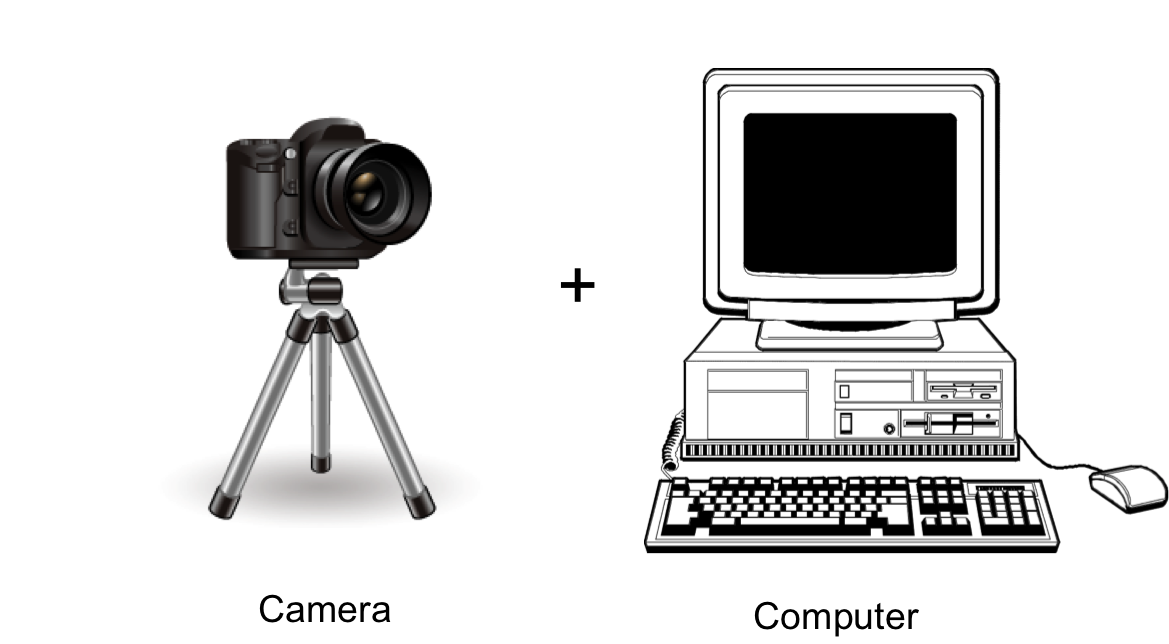
\includegraphics[width=.7\textwidth]{experimental_setup.png}
                \caption{Experimental setup consists of a good camera, a tripod, and a computer system. The camera captures images under pre-defined settings such as focal length, shutter speed, aperture size and luminance, while the computer is used to perform image enhancement \& filter analysis.}
\label{fig:exp_setup}                
\end{figure}

\noindent Our analysis architecture is designed to meet the following objectives:
\begin{enumerate}
\item  Retrieve sharper images using different filters and blur kernels. Train images are blurred using simulated standard point spread functions (PSF) and gaussian white noise of a specified variance is added. The obtained filter kernels are then compared against the kernel used to blur the image and the results are used to benchmark filter performance for the initially guesses PSF and noise variance. 
\item Generally, the sharpness of an image is determined by human visual systems. This process can be automated and made simpler if there was a robust metric to evaluate the sharpness of a restored image, and thus decide the optimum filter to restore a particular set of images. Before moving forward to automating the process of image sharpening, its important to understand the criteria and its limitations. For this purpose, three different sharpness metrics have been implemented and the criteria used has been tested against train images to understand its behavior. Finally, an automated function has been implemented and tested on an experimentally obtained image. The results are promising, but further development is required to make the function fully automated.

\end{enumerate}